\documentclass[a4paper,10pt]{article}
\usepackage[cm]{fullpage}
\usepackage[all]{xy}
\usepackage{natbib}
\usepackage{tikz}
\usepackage{booktabs}

\usepackage{amsmath,amssymb}
\usepackage{hyperref}

\usepackage{graphicx}

\newcommand{\argmin}{\operatorname*{arg\, min}}
\newcommand{\sign}{\operatorname{sign}}
\newcommand{\RR}{\mathbb R}
\newcommand{\NN}{\mathbb N}

\DeclareMathOperator*{\maximize}{maximize}

\begin{document}

\title{Supervised, interactive genomic data analysis
}
\author{
  Toby Dylan Hocking
}

\date{Barbados workshop, 5--9 Jan 2015}

\maketitle

\thispagestyle{empty}% needs to be after maketitle.
\pagestyle{empty}

\section*{Unsupervised, non-interactive
  DNA copy number profile analysis}

Approximate copy number as a function of genomic position can be
measured by array comparative genomic hybridization (aCGH), single
nucleotide polymorphism (SNP) microarrays, or whole-genome short-read
sequencing experiments.

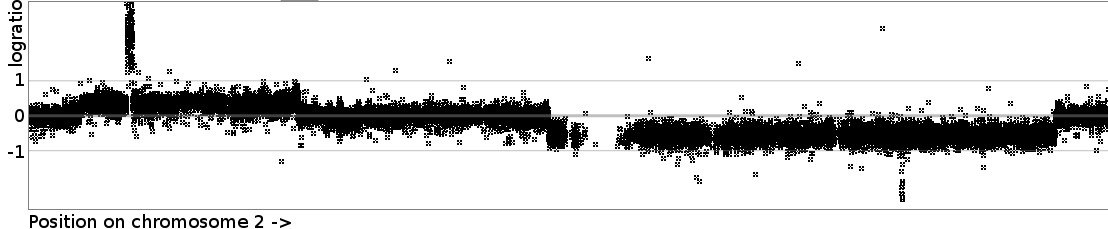
\includegraphics[width=\textwidth]{unlabeled-axes}

Goal: estimate the true locations of breakpoints, losses,
deletions, gains, and amplifications. (\textbf{unknown!})

\section*{Supervised, non-interactive
 analysis using annotated regions}

We can draw a set of annotated regions that encode our interpretation
of these data:

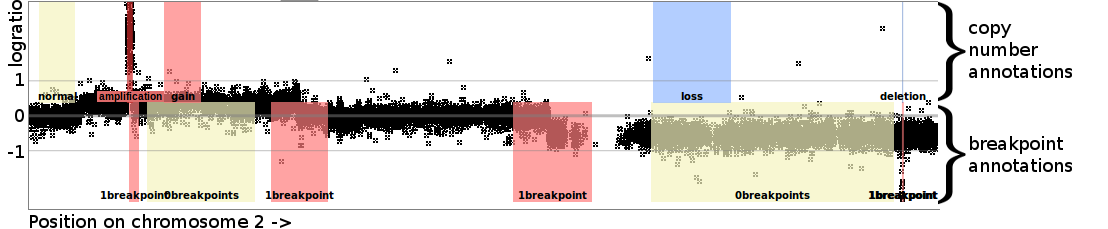
\includegraphics[width=\textwidth]{regions-axes-full}

Goal: use the probe logratios along with a subset of labeled regions
to train a model for accurate prediction on unlabeled
regions. (\textbf{Quantify accuracy using cross-validation --- set
  aside some labels as a test set!})

\section*{Supervised, interactive analysis on SegAnnDB
  \citep{HOCKING-SegAnnDB}}

Every time the set of annotated regions changes, the displayed model
is updated to agree. The model can be iteratively updated until it
matches your expert interpretation.

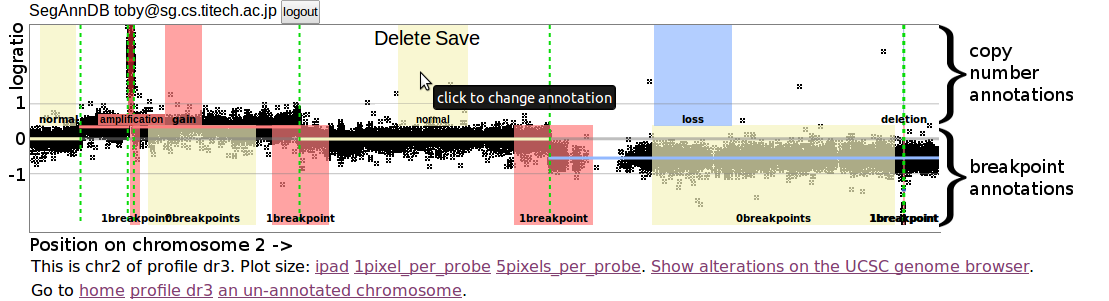
\includegraphics[width=\textwidth]{new-new-annotations}

\newpage

\section*{Unsupervised, interactive analysis}
\begin{displaymath}
  \xymatrix@=0.3cm{
    \text{Data $\mathbf x$}
    \ar `[r] [dr] 
    \ar `r[rr] [drr] 
    \ar `r[rrr] [drrr] 
    % \ar [d]
    & \text{ }
    & \text{ }
    & \text{ }
    \\
    % \text{Plot} 
    % \ar [d]
    & 
    \text{Model $f(\mathbf x, \lambda_1)$} 
    \ar [r]
    & 
    \textcolor{red}{\text{Plot}}
    \ar[d]
    &
    \text{Model $f(\mathbf x, \lambda_2)$} & \dots
    \\
    \text{Parameter $\lambda_1$}
    \ar `r[ru] [ru]
    \ar [rr]
    & \text{ }
    & \textcolor{red}{\text{Parameter $\lambda_2$}}
    \ar `r[ru] [ru] \\
    & &   \textcolor{red}{\text{Plot after modeling.}}
  }
\end{displaymath}

\section*{Supervised, interactive analysis}
% \begin{displaymath}
%   \xymatrix@=0.3cm{
%     \text{Data $\mathbf x$}
%     \ar `[r] [dr] 
%     \ar [d]
%     & \text{ }
%     \\
%     \textcolor{red}{\text{Plot} }
%     \ar [d]
%     & 
%     \text{Model $f(\mathbf x, \lambda)$} 
%     \\
%     \textcolor{red}{\text{Labels $\mathbf y$}       }
%     \ar [d]
%     \\
%     \textcolor{red}{\text{Parameter $\lambda$} }
%     \ar `r[ruu] [ruu]
%     & \text{ }\\
%     \textcolor{red}{\text{Plot before modeling.}}
%   }
% \end{displaymath}

\begin{displaymath}
  \xymatrix@=0.3cm{
    \text{Data $\mathbf x$}
    \ar `[r] [dr] 
    \ar `r[rr] [drr] 
    \ar `r[rrr] [drrr] 
    \ar [d]
    & \text{ }
    & \text{ }
    & \text{ }
    \\
    \textcolor{red}{\text{Plot 1} }
    \ar [d]
    & 
    \text{Model $f(\mathbf x, \lambda_1)$} 
    \ar [r]
    &
    \textcolor{red}{\text{Plot 2} }
    \ar [d]
    & 
    \text{Model $f(\mathbf x, \lambda_2)$}  & \dots
    \\
    \textcolor{red}{\text{Labels $\mathbf y_1$}       }
    \ar [d]
    \ar [rr]
    \ar [rru]
    &
    &
    \textcolor{red}{\text{Labels $\mathbf y_2$}}
    \ar [d]
    \\
    \textcolor{red}{\text{Parameter $\lambda_1$} }
    \ar `r[ruu] [ruu]
    & \text{ }
    & \textcolor{red}{\text{Parameter $\lambda_2$}}
    \ar `r[ruu] [ruu] \\
    \textcolor{red}{\text{Plot before modeling}} &
    &
    \textcolor{red}{\text{Plot after modeling}} 
  }
\end{displaymath}

Two differences:
\begin{itemize}
\item Labels $\mathbf y$ can be used for training parameters $\lambda$
  and testing models $f(\mathbf x, \lambda)$.
\item When to plot? \textbf{Before} and after fitting a model
  $f(\mathbf x, \lambda)$.
\end{itemize}

\section*{Summary of (un)supervised, (non-)interactive analysis}

  \begin{center}
  \begin{tabular}{c|c|c}
    Evaluation: & qualitative &  quantitative \\
    Input: profile $\mathbf x$ + & parameters $\lambda$ & labels $\mathbf y$ \\
        & \textbf{unsupervised} & \textbf{supervised}\\
    \hline
    \textbf{non-interactive}
    & plot $\mathbf x$ & plot $\mathbf x, \mathbf y$\\
    fit one model
    & default parameters $\lambda$ & trained parameters $\lambda$ \\
    & e.g. mBIC \citep{mBIC} & \citep{HOCKING-penalties, HOCKING-breakpoints}\\
    && ChIP-seq \citep{hocking2014visual}\\
    \hline
    \textbf{interactive}
    & plot $\mathbf x, f(\mathbf x, \lambda)$ 
    & plot $\mathbf x, \mathbf y, f(\mathbf x, \lambda)$\\
    plot, update model 
    & manually tuned $\lambda$ & iterative $\lambda$ training\\
    & e.g. CGHweb \citep{CGHweb}  & SegAnnDB \citet{HOCKING-SegAnnDB}
  \end{tabular}
  \end{center}

\bibliographystyle{abbrvnat}
\bibliography{refs}


\end{document}
